% document formatting
\documentclass[10pt]{article}
\usepackage[utf8]{inputenc}
\usepackage[left=1in,right=1in,top=1in,bottom=1in]{geometry}
\usepackage[T1]{fontenc}
\usepackage{xcolor}

% math symbols, etc.
\usepackage{amsmath, amsfonts, amssymb, amsthm}

% lists
\usepackage{enumerate}

% images
\usepackage{graphicx} % for images
\usepackage{tikz}

% code blocks
% \usepackage{minted, listings} 

% verbatim greek
\usepackage{alphabeta}

\graphicspath{{./assets/images/Week 7}}

\title{02-613 Week 7 \\ \large{Algorithms and Advanced Data Structures}}
 
\author{Aidan Jan}

\date{\today}

\begin{document}
\maketitle

\section*{Amortized vs. Average}
Recall that average refers to events in isolation and amortized refers to across the whole run.  We have used this for runtime analysis multiple times:
\begin{itemize}
    \item Tree traversal (BFS/DFS): It takes $|V| + |E|$ to run a traversal on a graph, but if we have a tree, we only run on a subset of edges.  Therefore we don't pay the cost of running on the whole graph.
    \item Heap insert: It takes $O(\log(n))$ to add a node to a heap, but not every node will take that long.  If we know the dataset, it can be lower.
\end{itemize}

\subsection*{Binary Increments}
Suppose we are counting in binary.  To go from $0$ to $1$, we flip 1 bit.  From $1$ to $2$, we flip 2 bits.  From $2$ to $3$, we flip 1 bit again.  But from $3$ to $4$, we flip 3 bits.
\begin{itemize}
    \item In the worst case, notice that we flip $k$ bits.  However, we would not say that flipping bits in binary is O($k$), because we \textit{know} that not every bit is flipped every iteration.
    \item Claim: cost to increment from 1 to $k$ is $2k$.
    \begin{itemize}
        \item The idea is that we "prepay" $1 \rightarrow 0$ flips.  We know that whenever we flip a bit from $0$ to $1$, we will eventually flip it back from $1$ to $0$.
        \item On every increment, we flip exactly one bit from $0 \rightarrow 1$.  All others are $1 \rightarrow 0$, which have already been "paid" for.
        \item From this, we can show that each operation costs $2$, and not $\log(k)$, even though $\log(k)$ bits are flipped in the worst case.
        \item This improves our runtime estimate to O($k$) instead of O($k \log k$)
    \end{itemize}
\end{itemize}

\section*{Improving Linked Lists}
Why do we ever use linked lists if all its operations are slower than arrays?  For example. get, length, and replace in an array are all O(1), but linked list are all O($n$).  A linked list is just slower to use.
\begin{itemize}
	\item This is where the perfect skip list comes in!
	\item Start with a linked list
	\item Promote half the nodes to a higher "level"
	\item Keeps a "head", "sentinel" to mark front and back
	\item Each node is on between 1 + O($\log n$) levels
	\item Higher levels skip nodes
\end{itemize}
\begin{center}
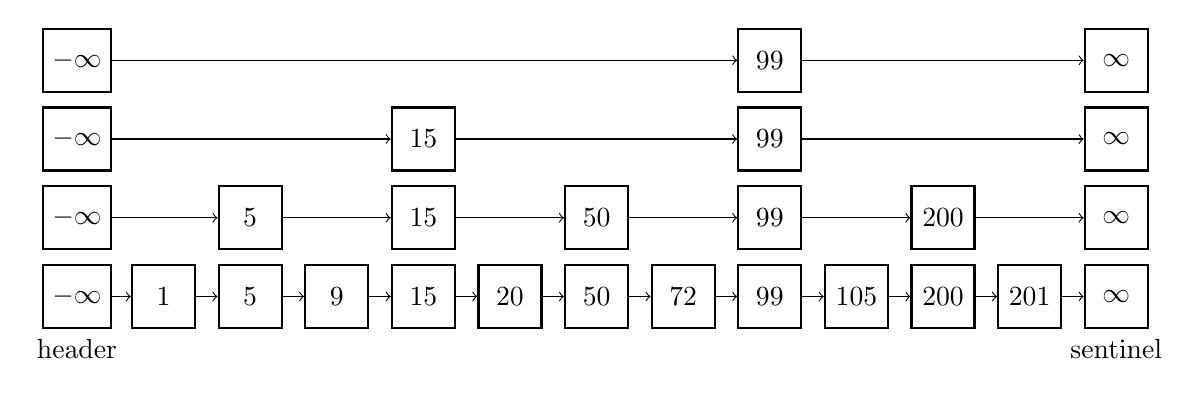
\begin{tikzpicture}
    \node[thick, draw, minimum width=0.8cm, minimum height=0.8cm, label=below:{header}] at (0, 0) (0) {$-\infty$};
    \node[thick, draw, minimum width=0.8cm, minimum height=0.8cm] at (1.1, 0) (1) {1};
    \node[thick, draw, minimum width=0.8cm, minimum height=0.8cm] at (2.2, 0) (2) {5};
    \node[thick, draw, minimum width=0.8cm, minimum height=0.8cm] at (3.3, 0) (3) {9};
    \node[thick, draw, minimum width=0.8cm, minimum height=0.8cm] at (4.4, 0) (4) {15};
    \node[thick, draw, minimum width=0.8cm, minimum height=0.8cm] at (5.5, 0) (5) {20};
    \node[thick, draw, minimum width=0.8cm, minimum height=0.8cm] at (6.6, 0) (6) {50};
    \node[thick, draw, minimum width=0.8cm, minimum height=0.8cm] at (7.7, 0) (7) {72};
    \node[thick, draw, minimum width=0.8cm, minimum height=0.8cm] at (8.8, 0) (8) {99};
    \node[thick, draw, minimum width=0.8cm, minimum height=0.8cm] at (9.9, 0) (9) {105};
    \node[thick, draw, minimum width=0.8cm, minimum height=0.8cm] at (11, 0) (10) {200};
    \node[thick, draw, minimum width=0.8cm, minimum height=0.8cm] at (12.1, 0) (11) {201};
    \node[thick, draw, minimum width=0.8cm, minimum height=0.8cm, label=below:{sentinel}] at (13.2, 0) (12) {$\infty$};

    \node[thick, draw, minimum width=0.8cm, minimum height=0.8cm] at (0, 1) (0a) {$-\infty$};
    \node[thick, draw, minimum width=0.8cm, minimum height=0.8cm] at (2.2, 1) (2a) {5};
    \node[thick, draw, minimum width=0.8cm, minimum height=0.8cm] at (4.4, 1) (4a) {15};
    \node[thick, draw, minimum width=0.8cm, minimum height=0.8cm] at (6.6, 1) (6a) {50};
    \node[thick, draw, minimum width=0.8cm, minimum height=0.8cm] at (8.8, 1) (8a) {99};
    \node[thick, draw, minimum width=0.8cm, minimum height=0.8cm] at (11, 1) (10a) {200};
    \node[thick, draw, minimum width=0.8cm, minimum height=0.8cm] at (13.2, 1) (12a) {$\infty$};

    \node[thick, draw, minimum width=0.8cm, minimum height=0.8cm] at (0, 2) (0b) {$-\infty$};
    \node[thick, draw, minimum width=0.8cm, minimum height=0.8cm] at (4.4, 2) (4b) {15};
    \node[thick, draw, minimum width=0.8cm, minimum height=0.8cm] at (8.8, 2) (8b) {99};
    \node[thick, draw, minimum width=0.8cm, minimum height=0.8cm] at (13.2, 2) (12b) {$\infty$};

    \node[thick, draw, minimum width=0.8cm, minimum height=0.8cm] at (0, 3) (0c) {$-\infty$};
    \node[thick, draw, minimum width=0.8cm, minimum height=0.8cm] at (8.8, 3) (8c) {99};
    \node[thick, draw, minimum width=0.8cm, minimum height=0.8cm] at (13.2, 3) (12c) {$\infty$};

    \draw[->] (0) edge (1); \draw[->] (1) edge (2); \draw[->] (2) edge (3); \draw[->] (3) edge (4);
    \draw[->] (4) edge (5); \draw[->] (5) edge (6); \draw[->] (6) edge (7); \draw[->] (7) edge (8);
    \draw[->] (8) edge (9); \draw[->] (9) edge (10); \draw[->] (10) edge (11); \draw[->] (11) edge (12);

    \draw[->] (0a) edge (2a); \draw[->] (2a) edge (4a);
    \draw[->] (4a) edge (6a); \draw[->] (6a) edge (8a);
    \draw[->] (8a) edge (10a); \draw[->] (10a) edge (12a);

    \draw[->] (0b) edge (4b); \draw[->] (4b) edge (8b); \draw[->] (8b) edge (12b);

    \draw[->] (0c) edge (8c); \draw[->] (8c) edge (12c);
\end{tikzpicture}
\end{center}
\begin{itemize}
    \item We want to keep the sorted nature of this structure whenever nodes are inserted.  
\end{itemize}

\subsubsection*{Search}
\begin{itemize}
	\item Sorted allows us to search nodes in O($\log n$) time.  For example, to find 201, we start from the header, $-\infty$, then compare to 99.
    \begin{itemize}
	    \item $201 > 99$ (level 3), so we keep checking.  $201 < \infty$ so we move down a level (to level 2).  
        \item $201 < \infty$ (still) so we move down another level
        \item $201 > 200$ so we move across to the 200 (level 1) node.
        \item $202 = 201$, so we move across.  We're done!
    \end{itemize}
\end{itemize}

\subsubsection*{Insertion}
To insert, we first find the spot to insert on the first level, which contains every node.  Then, we randomly promote a levels on nodes.
\begin{itemize}
	\item Literally, insert node at level 1.  \texttt{while (coin\_flip == True): insert node to next level}.  This process repeats infinitely.
\end{itemize}

\subsubsection*{Analysis}
We always enter the structure from the highest level.  For the purposes of runtime analysis we will consider the path taken to get to a node.
\begin{itemize}
	\item Consider the backwards walk from any element.  We always want to go as high as possible to retrace our steps.
	\item The probability we go up on a step is $\frac{1}{2}$.  This means we can either go left or up, with a $50\%$ chance at either one.
	\item To get to the $log(n)$-th level, it will take $2\log n$ steps.
	\item With high probability, the average search time is O($\log n$)
\end{itemize}

\section*{Splay Trees}
The idea:
\begin{itemize}
	\item Modify a BST
	\item More frequently accessed nodes are placed near the top
	\item Simple to implement
	\item Amortized O($\log n$) lookup
\end{itemize}
We have the function \texttt{splay(T, k)}, which moves a given node $k$ to the root (with some asterisks).  Basically,
\begin{verbatim}
Splay(T, k):
    if k is in T:
        move k to the root
    else:
        either the inorder predecessor or ancestor moves to the root.
\end{verbatim}
To understand how the splay function would work, consider a binary search tree with $J$ as the root.  Suppose we have a node $k$ we would like to splay to the top.
\begin{itemize}
	\item To do this, if $k > J$, then set $k$ as the root, take the right subtree of $J$ and make it the right subtree of $K$, and append $J$ (along with the left subtree) to be the left child of $k$.
	\item In the opposite case, $k < J$, we do the similar thing with making $k$ the root, appending the left subtree of $J$ to be the left subtree of $k$, and appending $J$ and the right subtree to the right child of $k$.
	\item The result is a valid binary search tree with the desired node $k$ at the top.  However, it is not necessarily balanced.
\end{itemize}

\subsection*{Find Item}
To find the item, we splay the item we want to the top, and check if it is the root.

\subsection*{Concatenate Two Trees}
Suppose we have $T_1$ and $T_2$, and we would like to combine them in the splay tree.  How do we do that?
\begin{itemize}
	\item We want to note that the new root must be either the smallest node of the larger tree, or the largest node of the smaller tree.  This is because binary trees must have everything on the left smaller than the root, and everything on the right larger than the root.
	\item To do this, we simply run \texttt{Splay(T1, inf)} on the smaller tree.  Since the largest node in the tree is the closest to infinity out of everything else in the tree, it will propagate the largest node to the top.
	\item Now, make that node the root of both trees, and use the rest of the smaller tree as the left child.  The other tree becomes the right child.
\end{itemize}

\subsection*{So How does Splay() Work?}
We use a concept called "rotations".
\begin{center}
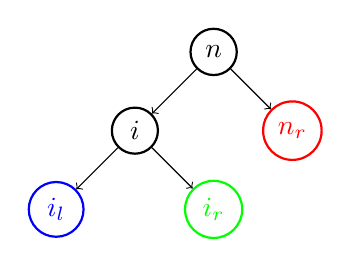
\begin{tikzpicture}
    \node[circle, thick, draw, blue] at (0, 0) (blue) {$i_l$};
    \node[circle, thick, draw, green] at (2, 0) (green) {$i_r$};
    \node[circle, thick, draw] at (1, 1) (i) {$i$};
    \node[circle, thick, draw, red] at (3, 1) (red) {$n_r$};
    \node[circle, thick, draw] at (2, 2) (n) {$n$};

    \draw[->] (n) edge (i);
    \draw[->] (n) edge (red);
    \draw[->] (i) edge (blue);
    \draw[->] (i) edge (green);
\end{tikzpicture}
\end{center}
Consider the following tree structure, where $n$ is the root, $i$ is the node we want to be the root, and $i_l$, $i_r$, and $n_r$ are the left and right subtrees of $i$ and the right subtree of $n$, respectively.
To "rotate" $i$ to the root, we make the structure the following:
\begin{center}
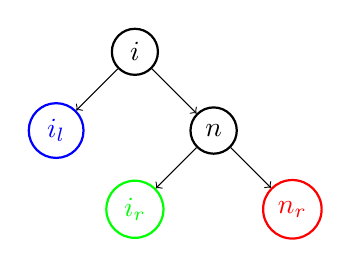
\begin{tikzpicture}
    \node[circle, thick, draw, blue] at (0, 1) (blue) {$i_l$};
    \node[circle, thick, draw, green] at (1, 0) (green) {$i_r$};
    \node[circle, thick, draw] at (1, 2) (i) {$i$};
    \node[circle, thick, draw, red] at (3, 0) (red) {$n_r$};
    \node[circle, thick, draw] at (2, 1) (n) {$n$};

    \draw[->] (i) edge (n);
    \draw[->] (n) edge (red);
    \draw[->] (i) edge (blue);
    \draw[->] (n) edge (green);
\end{tikzpicture}
\end{center}
Basically, we bubbled $i$ to the top, and since it was smaller than $n$ before, $n > i$, so $n$ becomes the right node.\\\\
In the opposite case, where $i$ was the right subchild to begin with, we get:
\begin{center}
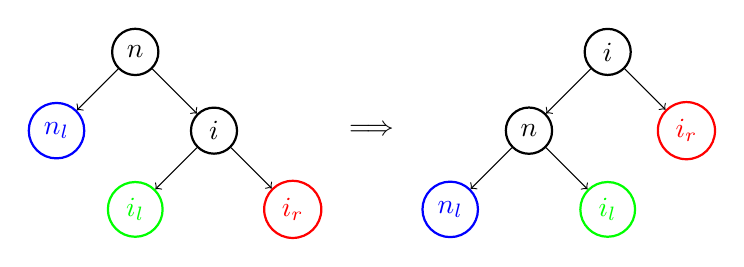
\begin{tikzpicture}
    \node[circle, thick, draw, blue] at (0, 1) (blue) {$n_l$};
    \node[circle, thick, draw, green] at (1, 0) (green) {$i_l$};
    \node[circle, thick, draw] at (2, 1) (i) {$i$};
    \node[circle, thick, draw, red] at (3, 0) (red) {$i_r$};
    \node[circle, thick, draw] at (1, 2) (n) {$n$};

    \draw[->] (n) edge (i);
    \draw[->] (i) edge (red);
    \draw[->] (i) edge (green);
    \draw[->] (n) edge (blue);

    \node[] at (4, 1) (text) {$\Longrightarrow$};

    \node[circle, thick, draw, blue] at (5, 0) (blue) {$n_l$};
    \node[circle, thick, draw, green] at (7, 0) (green) {$i_l$};
    \node[circle, thick, draw] at (7, 2) (i) {$i$};
    \node[circle, thick, draw, red] at (8, 1) (red) {$i_r$};
    \node[circle, thick, draw] at (6, 1) (n) {$n$};

    \draw[->] (i) edge (n);
    \draw[->] (n) edge (blue);
    \draw[->] (n) edge (green);
    \draw[->] (i) edge (red);
\end{tikzpicture}
\end{center}
A single rotation is called a \textbf{Zig}.

\subsubsection*{ZigZag}
A zig does not affect grandparents.  However, a zigzag does.  This operation is composed of basically two Zig operations
\begin{itemize}
    \item The first is on node (P), where (x) moves up and (P) becomes (x)'s left child.
    \item The second is on node (G), where (P) moves up and (G) becomes (P)'s right child.
\end{itemize}

\begin{center}
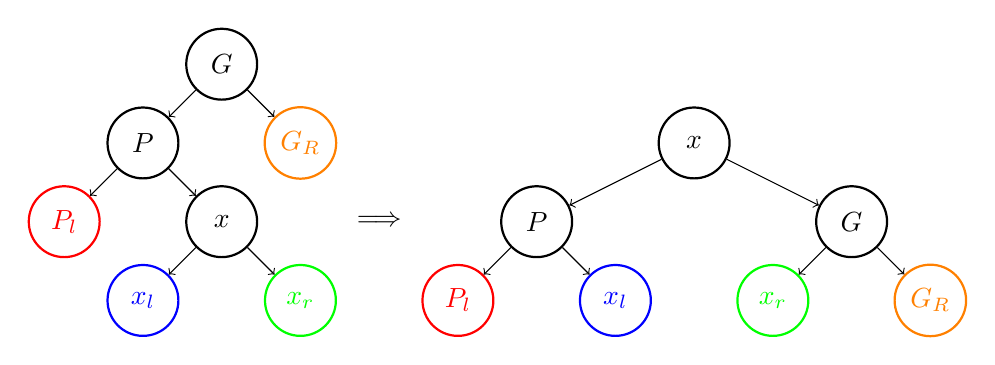
\begin{tikzpicture}
    \node[circle, thick, draw, red, minimum size=0.9cm] at (0, 1) (red) {$P_l$};
    \node[circle, thick, draw, blue, minimum size=0.9cm] at (1, 0) (blue) {$x_l$};
    \node[circle, thick, draw, green, minimum size=0.9cm] at (3, 0) (green) {$x_r$};
    \node[circle, thick, draw, minimum size=0.9cm] at (2, 1) (x) {$x$};
    \node[circle, thick, draw, minimum size=0.9cm] at (1, 2) (Px) {$P$};
    \node[circle, thick, draw, orange, minimum size=0.9cm] at (3, 2) (orange) {$G_R$};
    \node[circle, thick, draw, minimum size=0.9cm] at (2, 3) (P2x) {$G$};

    \draw[->] (P2x) edge (orange);
    \draw[->] (P2x) edge (Px);
    \draw[->] (Px) edge (red);
    \draw[->] (Px) edge (x);
    \draw[->] (x) edge (blue);
    \draw[->] (x) edge (green);

    \node[] at (4, 1) (text) {$\Longrightarrow$};

    \node[circle, thick, draw, red, minimum size=0.9cm] at (5, 0) (red1) {$P_l$};
    \node[circle, thick, draw, blue, minimum size=0.9cm] at (7, 0) (blue1) {$x_l$};
    \node[circle, thick, draw, green, minimum size=0.9cm] at (9, 0) (green1) {$x_r$};
    \node[circle, thick, draw, orange, minimum size=0.9cm] at (11, 0) (orange1) {$G_R$};
    \node[circle, thick, draw, minimum size=0.9cm] at (6, 1) (P1) {$P$};
    \node[circle, thick, draw, minimum size=0.9cm] at (10, 1) (G1) {$G$};
    \node[circle, thick, draw, minimum size=0.9cm] at (8, 2) (x1) {$x$};

    \draw[->] (x1) edge (G1);
    \draw[->] (x1) edge (P1);
    \draw[->] (G1) edge (green1);
    \draw[->] (G1) edge (orange1);
    \draw[->] (P1) edge (red1);
    \draw[->] (P1) edge (blue1);
\end{tikzpicture}
\end{center}

\subsubsection*{ZigZig}
This operation is also composed of two Zig operations:
\begin{itemize}
    \item The first is on node (G), where (P) moves up and (G) becomes (P)'s right child, resulting in a fully balanced tree.
    \item The second is on node (x), where (x) moves up and (P) becomes (x)'s right child.
\end{itemize}
\begin{center}
    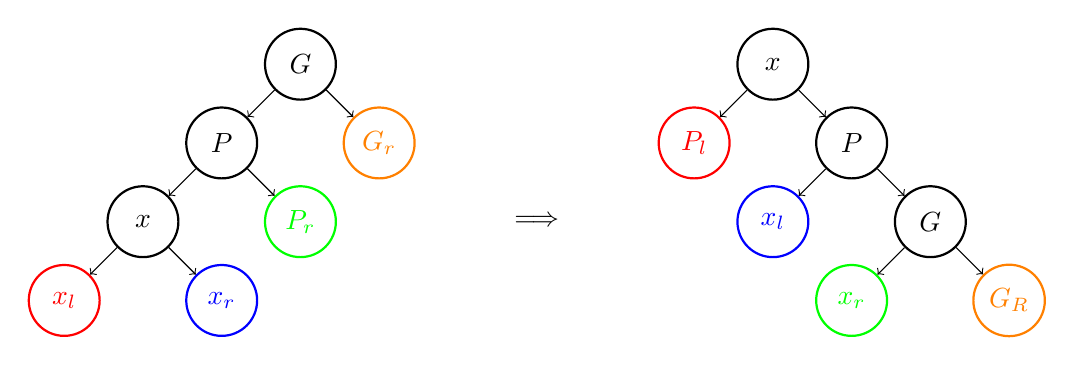
\begin{tikzpicture}
        \node[circle, thick, draw, red, minimum size=0.9cm] at (0, 0) (red) {$x_l$};
        \node[circle, thick, draw, blue, minimum size=0.9cm] at (2, 0) (blue) {$x_r$};
        \node[circle, thick, draw, green, minimum size=0.9cm] at (3, 1) (green) {$P_r$};
        \node[circle, thick, draw, minimum size=0.9cm] at (1, 1) (x) {$x$};
        \node[circle, thick, draw, minimum size=0.9cm] at (2, 2) (P) {$P$};
        \node[circle, thick, draw, orange, minimum size=0.9cm] at (4, 2) (orange) {$G_r$};
        \node[circle, thick, draw, minimum size=0.9cm] at (3, 3) (G) {$G$};
    
        \draw[->] (G) edge (orange);
        \draw[->] (G) edge (P);
        \draw[->] (P) edge (green);
        \draw[->] (P) edge (x);
        \draw[->] (x) edge (blue);
        \draw[->] (x) edge (red);
    
        \node[] at (6, 1) (text) {$\Longrightarrow$};
    
        \node[circle, thick, draw, red, minimum size=0.9cm] at (8, 2) (red1) {$P_l$};
        \node[circle, thick, draw, blue, minimum size=0.9cm] at (9, 1) (blue1) {$x_l$};
        \node[circle, thick, draw, green, minimum size=0.9cm] at (10, 0) (green1) {$x_r$};
        \node[circle, thick, draw, orange, minimum size=0.9cm] at (12, 0) (orange1) {$G_R$};
        \node[circle, thick, draw, minimum size=0.9cm] at (11, 1) (G1) {$G$};
        \node[circle, thick, draw, minimum size=0.9cm] at (10, 2) (P1) {$P$};
        \node[circle, thick, draw, minimum size=0.9cm] at (9, 3) (x1) {$x$};
    
        \draw[->] (x1) edge (red1);
        \draw[->] (x1) edge (P1);
        \draw[->] (P1) edge (G1);
        \draw[->] (P1) edge (blue1);
        \draw[->] (G1) edge (green1);
        \draw[->] (G1) edge (orange1);
    \end{tikzpicture}
    \end{center}

\subsection*{Cost of Splay}
What we really care about in runtime of the splay operation is the change of rank.
\begin{itemize}
    \item Assign every node in the tree with a weight, where weight is defined as the number of nodes in the subtree rooted at that node.  (e.g., all leaf nodes have weight 0)
    \item The rank of a node is defined as the floor of the log of its weight ($\text{rank}(u) \::= \lfloor \log \text{weight}(u) \rfloor$), and represents approximately how high up it is in the tree.
\end{itemize}

\textbf{Theorem:} It costs at most $3 \lfloor \log n \rfloor + 1$ new dollars to splay and keep the money invariant.
\begin{itemize}
	\item Each operation may be more expensive, but it can use savings.
\end{itemize}
Assume that we have the following costs for the varying splay operations:
\begin{itemize}
	\item Zig = $3(r^1(x) - r^0(x)) + 1$
	\item ZigZag = $3(r^1(x) - r^0(x))$
	\item ZigZig = $3(r^1(x) - r^0(x))$
\end{itemize}
In this case, $r^1$ refers to the rank of the parent, and $r^0$ refers to the rank of the child.  Why is this?
\begin{align*}
    &3(r^k(x) - r^0(x)) + 1 \\ 
    &\leq 3 r^k(x) + 1 \\
    &\leq 3 \lfloor \log(n) \rfloor + 1
\end{align*}
\begin{itemize}
	\item In the worst case, $r^0(x)$ is a leaf node, so the rank is 0.
	\item Also in the worst case, $r^k(x)$ is the root node, so the rank is $\log(n)$.
\end{itemize}
In the case of splaying multiple ranks, we have to use ZigZags and ZigZigs, so our total cost of the operation would be:
\[3(r^1(x) - r^0(x)) + 3(r^2(x) - r^1(x)) + \cdots + 3(r^k(x) - r^{(k - 1)}(x)) + 1\]
Where each term is to move subtrees up or down.
\begin{itemize}
	\item Refer to the costs described above.  The $+1$ at the end comes from the sole Zig operation at the end.
\end{itemize}

Now, how do we prove these costs are correct?
\subsubsection*{Proof}
First, we need a few lemmas:\\
\textbf{Lemma 1:} 
\[\text{cost}(\text{zig}) \leq 3(r^1(x) - r^0(x)) + 1\]
A zig needs $3(r^1(x) - r^0(x)) + 1$.  This relies on the fact that $r^0(P(x)) = r^1(x)$.  In other words, the total number of nodes below $P(x)$ in the original tree is equal to the number of nodes below $x$.  The $+1$ at the end pays for the actual rotation to swap the two nodes.\\\\
We can write the operations for a zig as
\[[r^1(x) + r^1(P(x))] - [r^0(x) + r^0(P(x))]\]
where the left represents the number of dollars needed on $x$ and $P(x)$, while the right represents the number of dollars we already have on $x$ or $P(x)$.  It is worth noting that $r^1(x)$ on the left term cancels the $r(P(x))$ in the right term, since they are equal.  Therefore, we can simplify:
\begin{align*}
    &= r^1(P(x)) - r^0(x) \\
    &\leq r^1(x) - r^0(x) \\
    &\leq 3[r^1(x) - r^0(x)]
\end{align*}
\textbf{Lemma 2:}
\[\text{cost}(\text{zigzig}) \leq 3(r^1(x) - r^0(x))\]
A zigzag needs $r^1(R) - r^0(x)$ new dollars.  $R$ refers to the grandparent node, and $S$ (which will be seen later) is the parent node we are doing the zigzag operation around.  In other words, $G \mapsto R$, $P \mapsto S$ in the diagrams above.\\\\
Assume that $r^1(R) = r^1(S) \cdot \alpha$, where $\alpha$ is defined as $\alpha = r^1(x) = r^0(R) = r^0(S) = r^0(x)$.  We know that
\begin{align*}
    2^\alpha &\leq w^1(R) \leq 2^{\alpha + 1} \\
    2^\alpha &\leq w^1(S) \leq 2^{\alpha + 1}
\end{align*}
Here, $\alpha$ is some constant, and $w$ is the weight of the node.  However, we know that
\[w^1(x) \geq w^1(R) + w^1(S)\]
because at the end, the node $x$ is at the top, and therefore its weight must be greater than that of both its children.  Therefore,
\[w^1(x) \geq 2 \cdot 2^\alpha = 2^{\alpha + 1} \Rightarrow r^1(x) = \alpha + 1\]
This is a contradiction since $r^1(x) \::= \alpha$.
\end{document}